\scanpage{14}

\figure{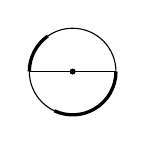
\begin{tikzpicture}[scale=.55]
\draw (0,0) circle (1);
\draw (-1,0)--(1,0);
\fill (0,0) circle (.07);
\draw[line width=1.2pt] (-1,0) arc (180:125:1);
\draw[line width=1.2pt] (1,0) arc (0:-115:1);
\end{tikzpicture}}

NB
\[
\mu_n=\operatorname{Ker}(G_m\xrightarrow{n}G_m)
\]
\[
\mu_n(X')=\deleted{\operatorname{Ker}}\,{}_n\Gamma(X',\mathcal O_{X'})^*
\]
\margin{$\mu_n$ fini plat sur $X$.}

Si $n$ premier aux car de $X$, $\mu_{nX}$ est \uline{étale} sur $X$
loc. isom. (pour top. étale) à $\mathbb Z/n\mathbb Z$. \unsure{Il n'faut|Il ne faut}
surtout pas les confondre. Les $\mu_{nX}^{\otimes d}$
($d\in\mathbb Z$) sont donc définis, et sont \inserted{loc} isomorphes à $(\mathbb Z/n\mathbb Z)_X$
[le choix d'une section primitive de $\mu_n$ définit des isom
$\mu_{nX}^{\otimes d}\simeq(\mathbb Z/n\mathbb Z)_X$, multipliant cette
section par $\lambda\in\mathbb Z/n\mathbb Z$ multiplie l'isom
précédent par $\lambda^d\ldots$].
\uline{Dém} presque immédiate par th. du changement de base\ldots

\margin{\fbox{Pureté ``absolue''}}
\uline{Pb} sans hypothèse de lissité remplacée par hyp.
de régularité. O.K. \inserted{pour \unsure{bons préschémas}}
pour corps car. \unsure{0} quand on
dispose de la résolution des singularités (Artin).

Il y a aussi un th de pureté relatif sur
une base quelconque\ldots

\deleted{13)}

\deleted{13) \uline{Les} $R^i_!f_*(F)$.}
\margin{Extension aux div. à croisements normaux\ldots}
\deleted{Morphismes \unsure{compactifiables} $f:X\longrightarrow Y$.
La factorisation
\diagram{\begin{tikzcd}
X\arrow[r,"i"]&\overline X\arrow[r,dash,"\bar f"]&\unsure{Y}
\end{tikzcd}},
où $i$ \unsure{imm.}}

\mspage{13}
